\section{研究背景和意义}
\label{sec:intro:backgroud}

%介绍什么是隐通道

%传统的时间隐通道,是利用数据的时间变化特性,承载目标数据。例如基于IP的时间隐通道(IP-CTC)[3].,基于回复时间的隐通道(TR-CTC)[4].,基于IPD的时间隐通道(IPD-CTC),利用数据包的长度变化规律来传送数据[10].,利用数据包之间的时间间隔(IPD)传送数据[12].,或者基于数据包分类的时间隐通道[13].,以及基于模型的时间隐通道(MB-CTC)[11].。

隐通道的明确定义,由Lampson在1973年提出\nupcite{4317620},隐通道是一种能够打破系统中的安全限制,允许低安全级别的进程访问高安全级别的数据。经过不断研究,隐通道不仅存在于单主机环境中,随着互联网应用范围的不断扩大,网络应用的不断丰富,隐通道的基础环境有了更多的候选项。根据构建方式的差异,隐通道可以划分为时间隐通道及存储隐通道两种类型,存储隐通道依赖于双方对相同存储位置的访问,时间隐通道依赖于双方对行为的观测。

\insertFigure{
	\begin{figure}
	    \centering
        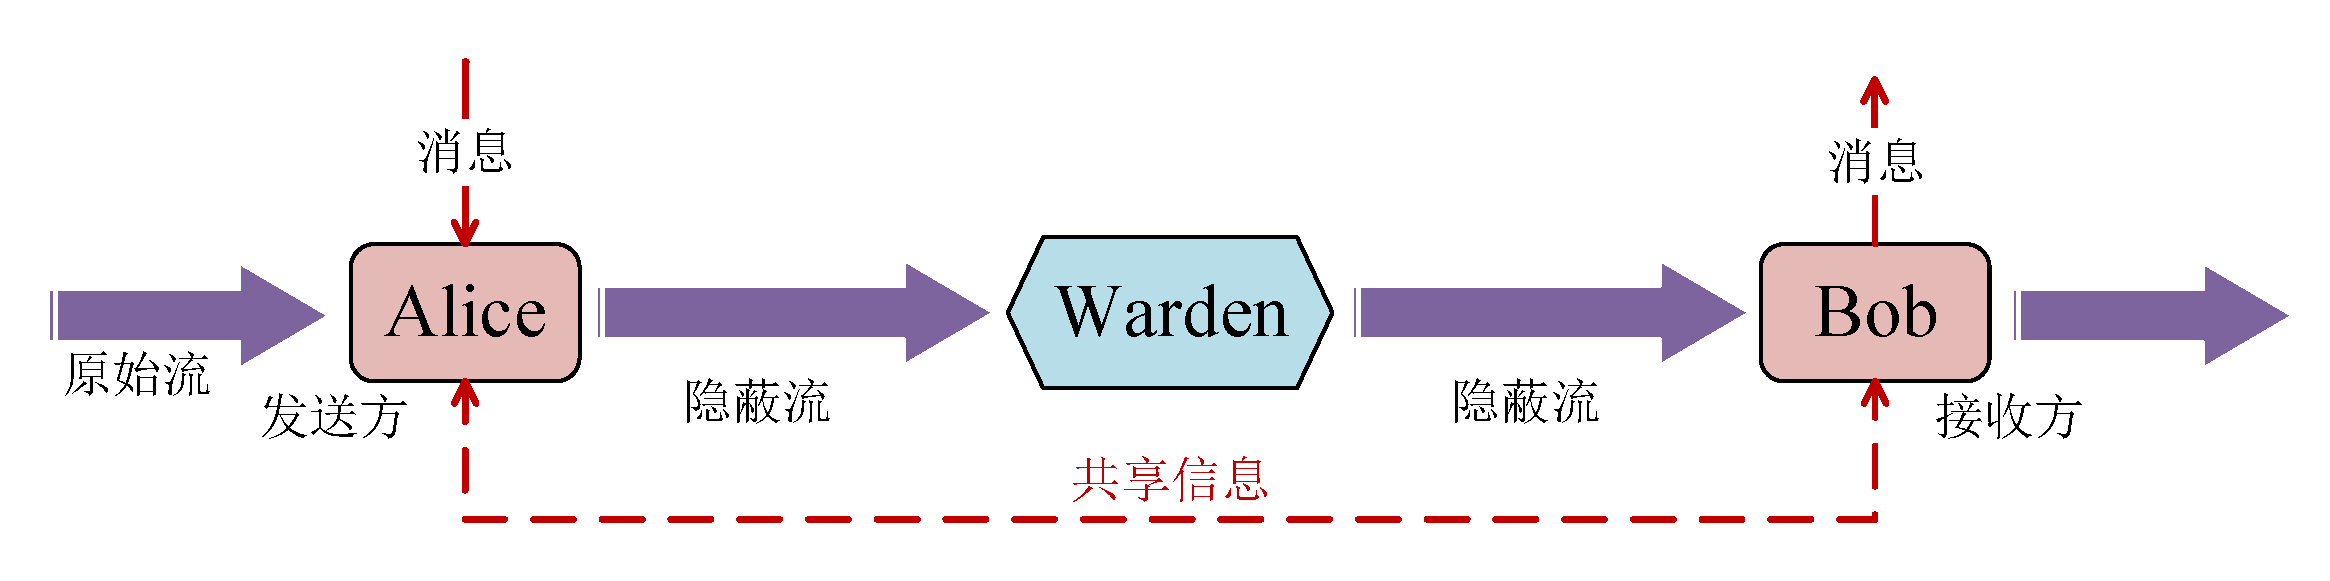
\includegraphics[width=\textwidth]{chapters/chapter1/figures/covert-channel.pdf}
        \caption{隐通道逻辑结构示意图}\label{fig:covert-channel}
	\end{figure}
}

对于隐通道的研究,主要集中在隐通道的构建方法和检测方法两个方面。隐通道的逻辑结构示意如图\nref{fig:covert-channel}所示,发送方和接收方利用共享信息,在发送方一侧将原始流调整为隐蔽流,由接收方识别隐蔽流中的特征,结合共享信息,提取出消息。

%时间隐通道相对存储隐通道的优势是什么
在不同的应用场景中,隐通道有多种表现形式。在单主机环境下,可以控制磁盘访问队列,利用磁盘响应时间构建存储隐通道\nupcite{130771};也可以利用键盘输入的

移动互联网的兴起

VoLTE是未来的趋势

研究VoLTE下时间隐通道构建方法,具有填补空白的意义
